\documentclass{article}
\usepackage{graphicx}
\graphicspath{ {/asay/Desktop/images/} }
\usepackage{color}
\usepackage{xepersian}


\title{پاسخ تمرین شماره ۲ درس معماری کامپیوتر}
\author{امیر حسین عاصم یوسفی \\ ۹۶۱۱۰۳۲۳}
\settextfont{B Nazanin}

\begin{document}
	\maketitle
	\section*{سوال ۱ : }
	برای حل این سوال باید به این توجه کرد که هر بلاک 
	$M$
	در واقع یک 
	$Carry \ Select \ Adder  \ (CSA)$
	می باشد که اندازه تاخیر آن برابر با مجموع تاخیر مالتی پلکسر ها و تاخیر 
	$CRA$
	ها می باشد که برای ۶۴ بیت به صورت زیر می باشد  : 
	\begin{center}
		$ D_{64\ bit\ adder } = D_{CRA} + ((\frac{64}{M}-1) \times D_{MUX}$
	\end{center}
همچنین باید این را در نظر گرفت که هر مالتی پلکسر یک تاخیر اضافه می کند (
$Fanout \ delay$
(
را اضافه می کند که این موضوع در تحلیل ما بسیار مهم است و به آن بر خواهیم گشت  . 
\\
حال اگر پیچیدگی های پیاده سازی واقعی صرف نظر کنیم و فرض کنیم که تاخیر هر 
$FA$
۱ بیتی 
$N$
برابر تاخیر یک مالتی پلکسر می باشد . بنابراین با توجه به تاخیر 
$CRA$
داریم  : 
\begin{center}
	$ D_{CRA} = N \times M \times D_{MUX}$\\
	$ D_{CRA } =(\frac{64}{M}-1) \times D_{MUX}$
\end{center}
با توجه به عبارت های بالا به معادله زیر می رسیم  : 
\begin{center}\textcolor{red}{(۱)}
	$NM^2 + M = 64$
\end{center}
که اگر در معادله بالا داشته باشیم 
$N=2$
(تاخیر هر جمع کننده ۱ بیتی۲ برابر تاخیر یک مالتی پلکسر می باشد ) آن گاه برای 
$M$
مقدار ۴۱.۵ به دست می آید که چون 
$M$
باید یک مقدار صحیح باشد می توان دو مقدار را برای آن در نظر گرفت که به شرح زیر می باشد  : 
\begin{center}
	$M = 5  \  , \ M = 6 $
\end{center}
که اگر مقدار ۵ را در نظر بگیریم این جمع در ۱۳ مرحله انجام می شود پس داریم : 
\begin{center}
	$D_{adder} = 2 \times 5  + 12  = 22 $
\end{center}
بنابراین به ازای این مقدار تاخیر ما به اندازه ۲۲ مالتی پلکسر می باشد . به طور مشابه این اتفاق به ازای مقدار ۶ نیز می افتد . \\
با توجه به چیزی که در اول درباره تاخیر مالتی پلکسر گفته شده می  توان فرض کرد که تاخیر یک جمع کننده ۱ بیتی برابر با تاخیر یک مالتی پلکسر با احتساب 
$Fanout \ Delay$
می باشد بنابراین معادله ۱ به شکل زیر تغییر می کند  : 
\begin{center}
	$1 \times M^2 + M = 64 $
\end{center}
که از معادله بالا مقدار ۵۲.۷ به دست می آید . که با توجه به این که 
$M$
باید یک مقدار صحیح داشته باشد مقدار 
\textcolor{red}{8}
را برای آن در نظر می گیریم که درآن صورت تاخیر ما به اندازه 
$8 \times 1  + 7  = 15$
مالتی پلکسر می باشد که مقدار مینیمم می باشد . \\
بنابراین به ازای 
$M = 8 $
به تاخیر مینیمم می رسیم  . 
\hrule
\section*{سوال۲ : }
kjdnvkjdfnvnvkkldjfnvav
\hrule
\section*{سوال ۳ : }
نتدسنیتبدنستیدبنتدسیبنتسد
\hrule
\section*{سوال ۴ : }
با توجه به این که هر چه قدر فرکانس کاری بالاتر رود زمان بین دو کلاک کمتر می شود بنابراین اگر فرکانس از حدی بالاتر رود طول کلاک ها برای انجام عملیات ها کافی نمی باشد  . \\
اگر بخواهیم حالتی از ضرب را در نظر بگیریم که به طولانی ترین کلاک نیاز دارد می توان حالتی را در نظر گرفت که یک عدد که هر ۳۲ بیت آن یک می باشد را در خودش ضرب کرد بنابراین در هر کلاک به عملیات ها زیر نیاز داریم  :‌
\begin{center}
	\begin{enumerate}
		\item به یک عملیات از سوی واحد کنترلی نیاز داریم که چک می کند ضرب شونده صفر شده است یا نه 
		\item بیت کم ارزش ضرب شونده را چک می کند 
		\item یک دستور جمع صادر می کند 
		\item یک عملیات جمع انجام می شود  
	\end{enumerate}
\end{center}
با توجه به این که تاخیر واحد کنترل برابر با ۸ می باشد در هر کلاک ۲۴ میکروثانیه نیاز داریم تا دستورات واحد کنترلی درهر کلاک به درستی انجام شود . \\
حال برای جمع کردن چون از یک 
$CSA$
۸ بیتی استفاده کرده ایم که با این واحد های ۸ بیتی می توان دو عدد ۳۲ بیتی را در ۴ مرحله جمع کرد و با توجه به فرمول  تاخیر زیر  : 
\begin{center}
	$ D_{CSA} = (\frac{n}{k}) \times D_{FA} + (k-1)\times D_{MUX}$
\end{center}
داریم  :  
\begin{center}
	$ k =  4 \  , \ n = 32 \ , \ D_{FA} = 5 \mu s \ , \ D_{MUX} = 4 \mu s \Rightarrow$\\
	$D_{CSA} = (\frac{32}{4})\times 5 + (4-1)\times 4  = 40 + 12 = 52 \mu s$
\end{center}

بنابراین ۵۲میکروثانیه هم برای انجام شدن دستور جمع در هر کلاک نیاز داریم پس  : 
\begin{center}
	$D_{Total} = 52 + 24 = 76 \mu s $
\end{center}
بنابراین طول هر کلاک باید ۷۶ میکروثانیه باشد تا  عملیات ضرب به درستی  انجام شود . ولی چون هم ضرب شونده و هم ضرب کننده ۳۲ بیتی هستند باید این مدار با فرکانسی کار کند که در ۳۲ کلاک بتواند کار را به اتمام برساند زیرا این مدار تا زمانی به کار خود ادامه می دهد که ضرب شونده صفر نشده باشد . \\

و با توجه به این که  
\begin{center}
	$Clock  \  Cycle \  Time = 76  \ \mu s = \frac{1}{Clock  \ Rate}$
\end{center}
بنابراین حداکثر فرکانسی که می تواند با آن کار کند برابر است با 
\begin{center}
	$Clock \ Rate  =  \frac{1}{76 \times 10 ^{-6}} \cong 13157Hz $
\end{center}
بنابراین با حداکثر فرکانس بالا کار کند  . 
\hrule
\section*{سوال ۵ : }
اگر هر کدام از اعداد 
$A$ 
و 
$B$
را به فرم زیر تعریف کنیم  : 
\begin{center}
	$A = X_{N}X_{N-1}X_{N-2}........X_{1}X_{0}$\\
	$B = Y_{N}Y_{N-1}Y_{N-2}.........Y_{1}Y_0$
\end{center}
حال با توجه به این که در الگوریتم ضرب ترکیبی هر بیت عدد 
$A$ 
را با هر بیت عدد 
$B$
، 
$AND$ 
می کنیم پس به 
\textcolor{red}{$N \times N = N^2$}
گیت 
$AND$
نیاز داریم  . \\
بعد از 
$AND$
کردن این اعداد آن ها را با یک دیگر جمع می کنیم که بنابراین به 
\textcolor{red}{$N(N-1)$}
جمع کننده (
$FA$
)
نیاز داریم ینابراین تعداد 
$HA$
ها برابر است با 
\begin{center}
	$N(N-1)\times 2 $
\end{center}
بنابراین با توجه به این محاسبات برای یک ضرب کننده ترکیبی ۴ بیتی مقادیر به شکل زیر می باشد  : 
\begin{center}

	$FA = 12 \Rightarrow HA = 12 \times 2  = 24 $\\
	 $AND \ Gate = 4 \times 4  = 16 $\\
\end{center}
بنابراین با توجه به این تاخیر گیت 
$AND$
برابر با ۳ واحد می باشد و این که تاخیر یک 
$HA$
برابر با ۴ واحد می باشد بنابراین تاخیر یک ضرب کننده  ترکیبی ۴ بیتی برابر است با  : 
\begin{center}
	$ D_{4bit \ Combinational \ Multiplier } = 24 \times 3 + 16 \times 4 = 72 + 64 = 136$
\end{center}
بنابراین تاخیر برابر با 
\textcolor{red}{136}
واحد زمانی می باشد  . 
\hrule
\section*{سوال ۶ : }
با توجه به فرمول تاخیر 
$Multi \ stage \ CSA $
که به شرح زیر می باشد  : 
\begin{center}
	$ D_{CSA} = (\frac{n}{k})\times D_{FA} + (k-1)\times D_{Mux}$
\end{center}
و همچنین با توجه به فرمول مساحت که به شرح زیر است : 
\begin{center}
	$ A_{CSA} = n \times ((\frac{2k-1}{k}))\times A_{FA} + (k-1) \times A_{Mux}$
\end{center}
حال با ضرب دو مقدار به دست آمده در بالا به یک تابع دو متغیره بر حسب متغیرهای 
\lr{n }
و  
\lr{k}
می رسیم که به صورت زیر می باشد  : 
\begin{center}
	$D_{CSA} \times A_{CSA} = ((\frac{n}{k})\times D_{FA} + (k-1) \times D_{Mux}) \times (n \times (\frac{2k-1}{k}) \times A_{FA} + (k-1) \times A_{Mux})  $
\end{center}
که برای سادگی می توان 
\lr{(k-1)}
را 
\lr{k}
در نظر گرفت و مقدار 
\lr{2k-1}
را 
\lr{2k}
در نظر گرفت پس تابع دو متغیره ما به صورت زیر ساده می شود  ‌ :
\begin{center}
	$D_{CSA} \times A_{CSA} = ((\frac{n}{k})\times D_{FA} + (k) \times D_{Mux}) \times (n \times (\frac{2k}{k}) \times A_{FA} + (k) \times A_{Mux}) $
\end{center}
که با انجام دادن این ضرب داریم : 
\begin{center}
	$H(n , k ) =  (\frac{2n^2}{k}) D_{FA} A_{FA} + nD_{FA}A_{Mux} + 2nk D_{Mux}A_{FA} + K^2A_{Mux}D_{Mux}$
\end{center}
اگر تابع دو متغیره بالا را بر حسب 
\lr{k}
کمینه کنیم به تعداد مراحلی می رسیم که 
\lr{area   * delay}
کمینه می شود  . پس بر حسب 
\lr{k}
 مشتق می گیریم برابر با صفر قرار میدهیم : 
 \begin{center}
 	$\frac{\partial H}{\partial  k} = (-\frac{2n^2}{k^2})D_{FA}A_{FA} + 2nD_{Mux}A_{FA} + 2kA_{Mux}D_{Mux} =0    $
 \end{center}
که از این معادله مقدار 
 \lr{k}
 برابر است با 
 ۲۵.۲
 که چون باید مقدار آن یک عدد صحیح باشد بنابراین مقدار 
 \textcolor{red}{2}
 را برای آن در نظر می گیریم  . \\
 بنابراین تاخیر یک جمع کننده ۸ بیتی برابر است با :
 \begin{center}
 	$D_{CSA} = (\frac{n}{k})\times D_{FA} + (k-1) \times D_{Mux}  \  , \ n = 8 , \ k = 2 \  , D_{Mux} = 3  ,D_{FA} = 3 \Rightarrow D_{CSA} = 15$
 \end{center}
\hrule
\section*{سوال ۷ : }
برای 
\lr{CLA}
داریم  : 
\begin{center}
 $P_i = X_i \oplus Y_i$\\
 $G_i  = X_i  . Y_i$\\
 $C_{i+1} = G_i + P_iC_i$\\
 $S_i = P_i \oplus C_i$
\end{center}
و با توجه به دوعدد داده شده داریم  : 
\begin{center}
	$ x _ 0 = 0  ,  \ x _1 = 1 \ , \  x_2 = 1 \ , \ x_3 = 0$\\
	$y_0 = 1  \ , \ y_1 = 0 \ , \ y_2 = 0  \ , \ y_3 = 1 $
\end{center}
بنابراین برای 
$P_i$
ها داریم  : 
\begin{center}
	$P_0 = x_0 \oplus y_0  = 1 $\\
	$P_1 = x_1 \oplus y_1  = 1 $\\
	$P_2 = x_2 \oplus y_2  = 1 $\\
	$P_3 = x_3 \oplus y_3  = 1 $
\end{center}
برای 
$G_i $
ها داریم  : 
\begin{center}
	$ G_0 = x_0 . y_0 = 0$\\
	$ G_1 = x_1 . y_1 = 0$\\
	$ G_2 = x_2 . y_2 = 0$\\
	$ G_3 = x_3 . y_3 = 0$
\end{center}
برای 
$C_i$
ها داریم  :
\begin{center}
	$C_0 = 1 \Rightarrow C_1 = G_0 + P_0C_0 = 1 $\\
	$C_2 = G_1 + P_1C_1 = 1$\\
	$C_3 = G_2 + P_2C_2 = 1$
\end{center}
\newpage
برای 
$S_i$
ها داریم  : 
\begin{center}
	$ S_0 = P_0 \oplus C_0 = 0$\\
	$ S_1 = P_1 \oplus C_1 = 0$\\
	$ S_2 = P_2 \oplus C_2 = 0$\\
	$ S_3 = P_3 \oplus C_3 = 0$
\end{center}
بنابراین 
\begin{center}
	\textcolor{red}{$C_3 = 1$} \\
	\textcolor{red}{$S_3 = 0$}
\end{center}
\hrule
\section*{سوال ۸ : }
\subsubsection*{قسمت اول  : }
مراحل کار هر ضرب کننده را می توان به صورت زیر تقسیم بندی کرد  : 
\begin{center}
	\begin{enumerate}
		\item تولید کردن ضرب های جزئی 
		\lr{(Partial Products)}
		\item جمع کردن ضرب های جزئی 
		\item جمع نهایی و به دست آوردن حاصل ضرب 
	\end{enumerate}
\end{center}
اما تمام تفاوت و برتری روش 
\lr{Wallace Tree}
در قسمت دوم نهفته است که ایده ی آن بر اساس 
\lr{Divide \& Conqure}
می باشد که به جای این که ضرب های جزئی را تک به تک با یک دیگر جمع کند از واحد های 
\lr{CSA (Carry Save Adder)}
استفاده می کند  . \\
مزیت های این روش به شرح زیر می باشد  : 
\begin{center}
	\begin{enumerate}
		\item سرعت بالا 
		\item توان مصرفی پایین 
		\item تاخیر کمتر 
		\item تعداد سطوح منطقی کمتری برای جمع کردن در آن وجود دارد 
	\end{enumerate}
\end{center}
هدف استفاده از این روش رسیدن به سرعت بیشتر و در عین حال داشتن توان کمتر می باشد و امروزه در بسیاری از موارد   مانند  محاسبات ممیز شناور و تحلیل و پردازش سیگنال کاربرد بسیار فراوانی دارد . 
\subsubsection*{قسمت دوم  : }
روش انجام آن به این شکل است که ابتدا بیت های 
\lr{Multipicant }
را با بیت های 
\lr{Multiplier}
تک به تک 
\lr{And}
کنیم تا به ضرب های جزئی برسیم و در مرحله با استفاده از 
\lr{CSA}
ها ضرب های جزئی را جمع می کنیم  و در نهایت برای جمع آخر از یک 
\lr{CPA (Carry Propagate Adder)}
استفاده می کنیم . \\
بنابراین برای طراحی چنین مداری که دو عدد ۴ بیتی را در یک ضرب کند به اجزای زیر نیاز داریم  : 
\begin{center}
	\begin{enumerate}
		\item گیت 
		\lr{AND}
		۱۶ عدد 
		\item جمع کننده 
		\lr{CSA}
	۵  عدد 
		\item جمع کننده 
		\lr{CPA}
		۱ عدد 
	\end{enumerate}

\end{center}
\subsubsection*{حاصل ضرب خواسته شده  : }
با توجه به شماره دانشجویی داریم  : 
\lr{Multiplier   = 323 \% 32  = 3 = $(0011)_2$ }
و با توجه به صورت سوال داریم  : 
\lr{Multipicant = $(1011)_2$}
\newpage
پس  : 
\begin{center}
	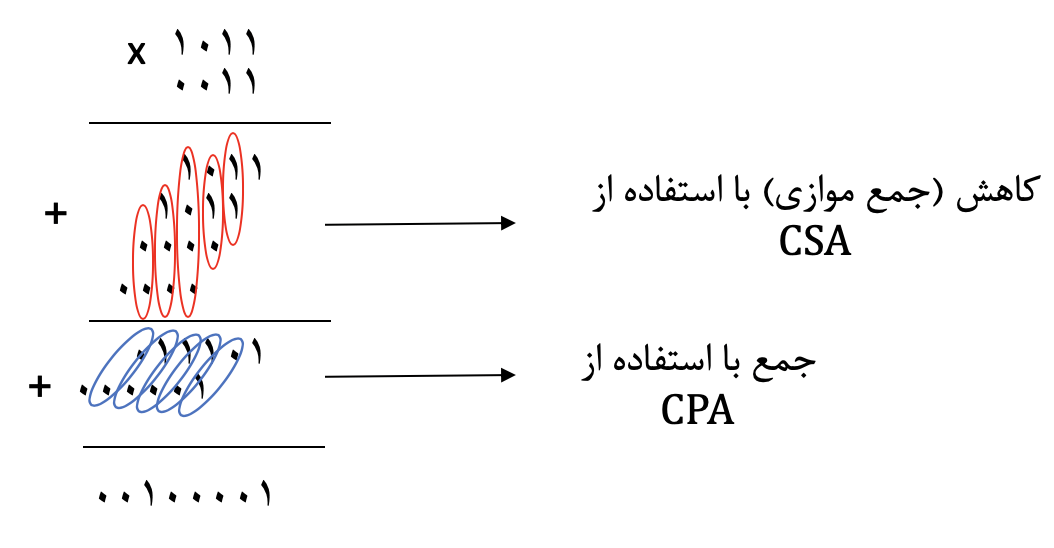
\includegraphics[width=1\textwidth]{wallace}
\end{center}
همان طور که می توان دید حاصل ضرب برابر با عدد ۳۳ (در مبنای ۱۰ ) می باشد . 
\hrule
\end{document}